% -*-coding: utf-8 -*-
% Держать в начале каждого файла!

\documentclass[a4paper, 12pt]{extarticle}
\usepackage{metod}

\MTDSetPhysSection{Механика}
\MTDSetTitle{Изучение закона сохранения энергии с~помощью маятника Максвелла}
\MTDDesignator{М--10}
\MTDSetGrade{10}

\MTDSetAuthors{И.~Н.~Грачева, В.~И.~Гребенкин, А.~Е.~Иванов, И.~А.~Коротова,
Е.~И.~Красавина, А.~В.~Кравцов, Н.~С.~Кулеба, Б.~В.~Падалкин,
Г.~Ю.~Шевцова, Т.~С.~Цвецинская}

\MTDSetEditorsGenCase{И.~Н.~Грачевой, А.~Е.~Иванова, А.~В.~Кравцова}

\newcommand{\eps}{\epsilon}

\begin{document}

\MTDTitlePage
\MTDInfoPage

\setcounter{section}{10}

\subsection{Цель работы}
Ознакомление со сложным движением твердого тела и изучение закона сохранения энергии на примере движения маятника Максвелла.

\subsection{Основные теоретические сведения}
Маятник Максвелла представляет собой металлический ролик "--- диск, насаженный на стержень, укрепленный на бифилярном  подвесе. Для изменения условий опыта даны сменные кольца, которые надеваются на диск. Если нити подвеса симметричным образом от концов стержня к диску намотать на стержень и освободить, то ролик начинает совершать сложное колебательное движение: поступательное вверх и вниз и вращательное вокруг оси симметрии. Считая, что нить не проскальзывает по стержню, можно ожидать, что изменение потенциальной энергии ролика при намотке нитей будет равно полной кинетической энергии маятника в низшей точке его траектории. Эта энергия состоит из двух составляющих: кинетической энергии поступательного движения центра масс маятника и кинетической энергии вращения его вокруг оси, проходящей через центр масс: %ИЗМ: убрала точку, поставила двоеточие
\[ %мб номер
W_\text{к} = \frac{mv^2 + I\omega^2}{2}. %ИЗМ: frac
\]

Начальная потенциальная энергия маятника %зачем тут новый абзац?; вынесла формулу, а то как-то несправедливо, мб и не надо этого делать
\[
W_\text{п} = mgh.
\]

Масса ролика складывается из массы стержня 0,019~\Units{кг} и массы диска 0,1~\Units{кг}. Массы колец определяются взвешиванием. Все размеры для вычисления момента инерции маятника определяются с помощью штангенциркуля. Момент инерции маятника, как и его масса, является аддитивной величиной. Он складывается из трех величин: %сделала itemize, мб не надо
\begin{itemize}
\item момента инерции стержня ролика $\dfrac{m_c r^2}{2}$
\item момента инерции диска ролика, насаженного на стержень, $\dfrac{m_D (r^2 + R^2)}{2}$
\item момента инерции съемного кольца $\dfrac{m_k(R_1^2 + R_2^2)}{2}$.
\end{itemize}

Для определения линейной и угловой скорости маятника воспользуемся системой уравнений динамики поступательного и вращательного движения и кинематической связи между угловыми и линейными характеристиками при движении без проскальзывания нити:
\begin{align*} %мб сделать как настоящую систему | Я бы не делал, мне кажется, что это будут скобки ради скобок
ma &= mg - 2T, \\ %я тут запятые добавила, но сомневаюсь, нужны ли они | Да, нужны
I \eps &= 2Tr, \\
a &= \eps r.
\end{align*}
Здесь  $m$ "--- масса маятника, $I$ "--- его момент инерции, $g$ "--- ускорение силы тяжести, $r$ "--- радиус стержня, $T$ "--- сила натяжения одной из нитей, $a$ "--- ускорение поступательного движения центра масс маятника, $\eps$ "--- угловое ускорение маятника.

Зная линейное и угловое ускорение маятника, найдем линейную и угловую скорость маятника в нижней точке его траектории:
\begin{align*}
v &= at, \\%опять запятая и точка
\omega &= \eps t.
\end{align*}

\subsection{Порядок выполнения работы}

\begin{figure}[h]
\centering
\begin{minipage}[b]{0.45\linewidth}
\centering
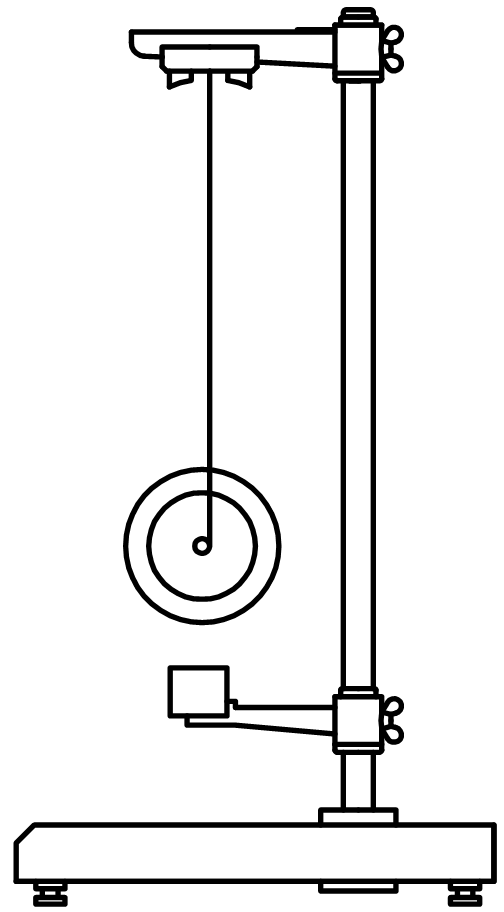
\includegraphics[scale = 0.3, keepaspectratio=true]{M10-MaxwellPendulumMachine}
\caption{\label{fig:m10-maxwell's-pendulum}}
\end{minipage} \hfill
\begin{minipage}[b]{0.45\linewidth}
\centering
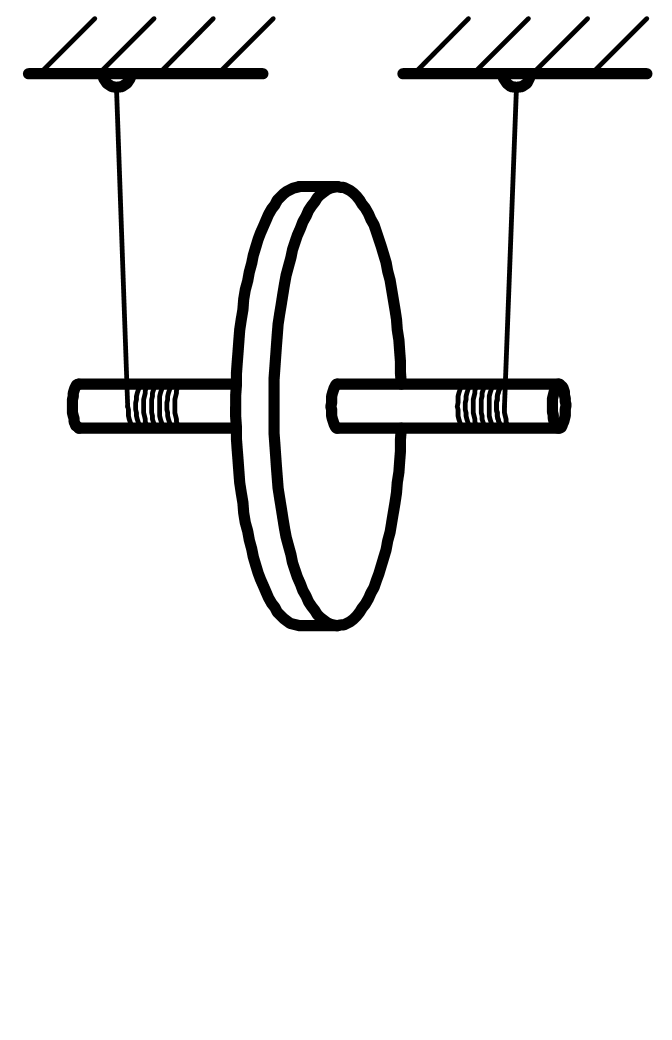
\includegraphics[scale = 0.2, keepaspectratio=true]{M10-MaxwellPendulum}
\caption{\label{fig:m10-wheel}}
\end{minipage}
\end{figure}

% Ты не думаешь, что стоило бы эти картинки в предыдущий сабсекшн?

% \MTDWarn{В целях сохранения симметрии тела маятника его нужно оберегать от ударов.} не уверена что это подходящий случай % Так и не пригодится мой маленький макрос :)
\textbf{Внимание!} В целях сохранения симметрии тела маятника его нужно оберегать от ударов. %сделала полужирным вместо подчеркивания
\begin{enumerate}
\item Собрать установку, укрепив нижний кронштейн с фотодатчиком в нижнее положение шкалы так, чтобы верхняя плоскость кронштейна совпала с одной из рисок шкалы. Основание установки отрегулировать с помощью опор так, чтобы подвешенный диск находился против центра окна фотодатчика. Нижний край диска должен находиться на 4--5~\Units{мм} ниже оптической оси фотодатчика. При этом ось ролика должна иметь строго горизонтальное положение.
\item Подключить фотодатчик и электромагнит, находящийся рядом с местом закрепления подвеса, к блоку питания. При включении кнопки <<сеть>> должно включиться табло индикации фотодатчика.
\item Симметрично наматывая нити маятника виток к витку от периферии к центру стержня ролика, закрепить его с помощью электромагнита в верхнем положении. В зафиксированном положении нити должны слегка провиснуть.
\item Нажав кнопку <<сброс>>, убедиться, что на табло индикатора установлены нули.
\item Нажатием кнопки <<пуск>> освободить ролик от электромагнита. В момент отключения электромагнита начинается отсчет времени движения таймером блока. Отсчет времени прекращается при перекрытии диском окна фотодатчика. \\
Время движения ролика $t$ и его ход $h$, определенный по шкале на стойке, занести в таблицу. Для повторения опыта нажать предварительно кнопку <<сброс>>.
\item По данным опыта определить относительную погрешность эксперимента для экспериментального и теоретического значения линейного ускорения:
\begin{align*}
a_\text{э} &= \frac{2h}{t^2}, \\%опять запятая и точка
a_\text{т} &= \frac{g}{1 + \frac{I}{mr^2}}, \\
\eps &= \frac{a_\text{э} - a_\text{т}}{a_\text{т}} \cdot 100 \%. %немного поменяла местами множители, добавила cdot
\end{align*}
\item По данным опыта вычислить кинетическую и потенциальную энергию маятника Максвелла в крайних положениях. Найти работу сил трения как разность их значений.
\end{enumerate}

\subsection{Контрольные вопросы}
\begin{enumerate}
\item Получить формулу момента инерции кольца массой $m$ с внутренним и внешним радиусами $R_1$ и $R_2$, пользуясь известной формулой для момента инерции диска и свойством аддитивности этой физической величины.
\item Вывести формулу для теоретического значения  ускорения центра масс маятника.
\item Как изменится ход рассуждений о сохранении и изменении механической энергии маятника Максвелла, если за нулевой уровень потенциальной энергии принять уровень верхнего, а не нижнего положения ролика?
\end{enumerate}

\end{document}
